% Chapter 6

\chapter{RESULTS} % Write in your own chapter title

\section{Results}
The proposed optimization is used on 4 different test cases. The relative improvement percentage (RIP) is the difference of optimization times between the two versions with and without applying the optimization. The optimization time is defined as the sum of both the compilation time and the running time.

\begin{equation*}
RIP(O) = \frac{T(O = 0) - T(O = 1)}{T(O = 1)} * 100 
\end{equation*}

If  $RIP  (O  =  0) \le 0$,  the  optimization has a negative effect, so it is better to not apply the optimization,

We evaluate our optimization with three different test cases which cover most use cases of our optimization

\subsection{Assessment}

\subsubsection{Test Case 1}

The Fibonacci sequence is used as the code for this test case. Traditional way of finding Fibonacci includes accessing two array indexes to calculate the successor. 

The results of applying our optimization are

\begin{figure}[H]
%	\centering
	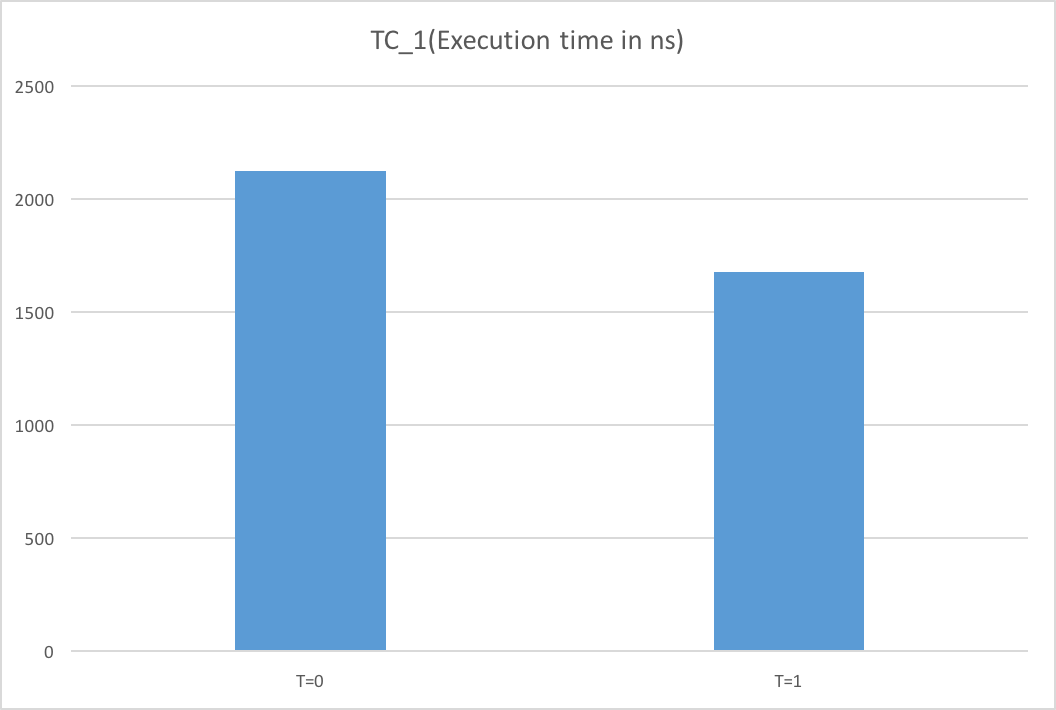
\includegraphics[scale=0.8]{tc_1.png}
	\caption{Execution times for TC 1}
	\label{TC_1}	
\end{figure}

\subsubsection{Test Case 2}

The optimization quality is proportional to the number of array accesses in the loop. This is depicted by this use case. 

The results of applying our optimization are

\begin{figure}[H]
	\centering
	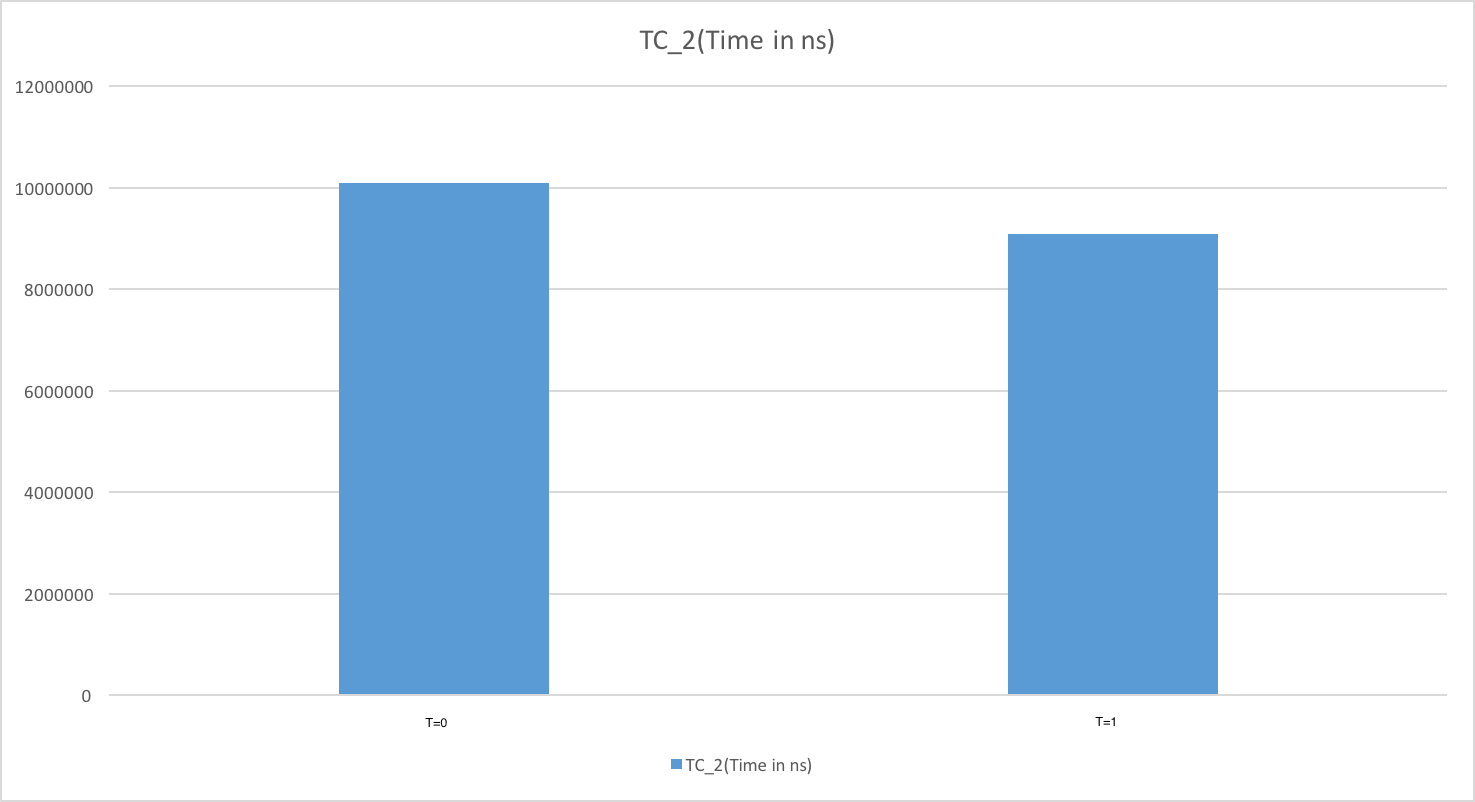
\includegraphics[scale=0.5]{tc_2.png}
	\caption{Execution times for TC 2}
	\label{TC_2}	
\end{figure}

\subsubsection{Test Case 3}

Not applying the optimization when not needed is also an evaluation of our system. Keeping this in mind, this test case contains code which cannot be optimized.

The results of applying our optimization are depicted in \ref{TC_3}

\begin{figure}[H]
	\centering
	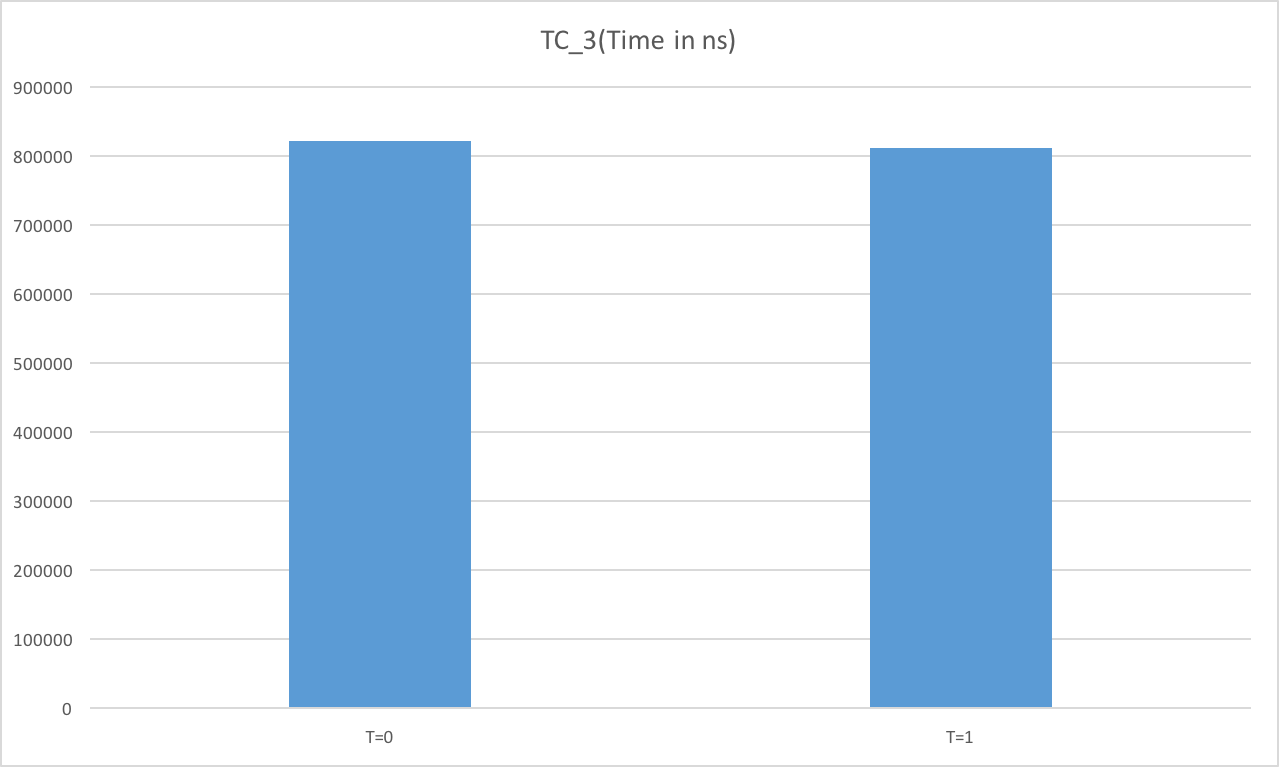
\includegraphics[scale=0.3]{tc_3.png}
	\caption{Execution times for TC 3}
	\label{TC_3}	
\end{figure}

\pagebreak

\subsection{Evaluation}

For each test case, we then find the RIP according to our formula. The results are below 

\begin{figure}[H]
	\centering
	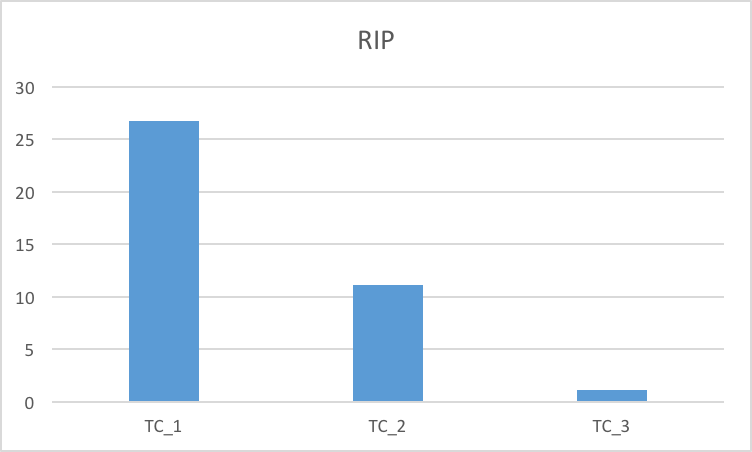
\includegraphics[scale=0.5]{rip.png}
	\caption{RIP of all test cases}
	\label{RIP}	
\end{figure}

We can deduce the following observations

\begin{enumerate}
	\item The performance is directly proportional to the number of array accesses present in the loop.
	\item There is no improvement or deterioration when the optimized is not applicable. 
\end{enumerate}
